\documentclass{article}
\usepackage[utf8]{inputenc}

\title{Idea in bullets}
\author{Vasilis Gkolemis}
\date{June 2021}

\usepackage{graphicx}
\usepackage{hyperref}
\usepackage{amsmath}
\usepackage{float}
\graphicspath{ {./../examples/} }

\begin{document}

\maketitle


\section{Intro}

ALE plots are the best feature effect (FE) technique, because ...
However, they have three drawbacks; Firstly, they do not provide
uncertainty about the measured effect, i.e.\ how confident to be that
the provided effect is the correct one. Secondly, in many cases, the
provide different effect depending on the number of bins (and we do
not have a measure to choose which one is closer to reality). Finally,
there are cases where it is impossible to create accurate ALE plots,
with fixed-size bins.


\section{Can we trust the ALE plot?}

In ALE, the user defines the bin-size, through one of the following
hyperparameters:

\begin{itemize}
\item \(K\), number of bins
\item \(dx\), bin-size
\item \(\texttt{min\_points\_per\_bin}\)
\end{itemize}
%
There is `1-1' relation between these hyperparameters:

\begin{equation*}
 dx \leftrightarrow K \leftrightarrow \texttt{min\_points\_per\_bin}
\end{equation*}
%
Therefore, we refer to them interchangeably.


\subsubsection*{Statement}

Altering the number of bins \( (K) \) leads to different ALE plots and
we do not have any indicator which plot is closest to the truth.

\subsubsection*{Example}

We define the following model:

\begin{equation} \label{eq:bullet-1-model}
  f(x_1, x_2) = x_1x_2 +
  \begin{cases}
    -5  + 0.3 x_1 &,  0  \leq x_1 < 20 \\
    1   + 7  (x_1 - 20) &,  20 \leq x_1 < 40 \\
    141 - 1.5(x_1 - 40) &,  40 \leq x_1 < 60 \\
    111 + 0  (x_1 - 60) &,  60 \leq x_1 < 80 \\
    111 - 5  (x_1 - 80) &,  80 \leq x_1 < 100
  \end{cases}
\end{equation}
%
where \(x_1 \perp x_2\) and \(x_2 \sim \mathcal{N}(\mu=0, \sigma=4)\).
Therefore, the gradients wrt. \(x_1\) are:

\begin{equation} \label{eq:bullet-1-data-effect}
  \frac{\partial f}{ \partial x_1} (x_1) = x_2 +
  \begin{cases}
    0.3 &,  0  \leq x_1 < 20 \\
    7   &,  20 \leq x_1 < 40 \\
    1.5 &,  40 \leq x_1 < 60 \\
    0   &,  60 \leq x_1 < 80 \\
    -5  &,  80 \leq x_1 < 100
  \end{cases}
\end{equation}
%
where \(x_2 \sim \mathcal{N}(\mu=0, \sigma=4)\). The ground truth ALE is:

\begin{equation} \label{eq:bullet-1-gt-ale}
  f_{\mathtt{ALE}}(x_s) = c +
  \begin{cases}
    -5  + 0.3 x_s &,  0  \leq x_s < 20 \\
    1   + 7  (x_s - 20) &,  20 \leq x_s < 40 \\
    141 - 1.5(x_s - 40) &,  40 \leq x_s < 60 \\
    111 + 0  (x_s - 60) &,  60 \leq x_s < 80 \\
    111 - 5  (x_s - 80) &,  80 \leq x_s < 100
  \end{cases}
\end{equation}
%
where \(c\) is a normalizing constant.

We generate N = 100 data points uniformly in the region \([0,100]\),
i.e., \(\mathcal{D} \sim \mathcal{U}(0, 100)\). The produced feature
effect plot is shown in figure \ref{fig:bullet-1-im-1}.

We observe that we get different plots for \(K=\{3, 5, 20, 100\}\),
without information which one to trust. If we set a threshold on
\(\texttt{min\_points\_per\_bin}\), then we discard plots (c) and (d)
beacuse they violate the threshold. In this case, among (a) and (b),
we cannot know which one to trust (We cannot trust both, since they
provide different effects).

For \(K=3\), the available resolution is smaller than the one
required, leading to an erroneous estimation. For \(K=5\), the feature
effect matches the correct resolution. For \(K=20, 100\), the feature
effect provides the general trend, but with noisy artifacts due to
small number of points per bin (violating
\texttt{min\_points\_per\_bin}).

\begin{figure}[!h]
  \centering
  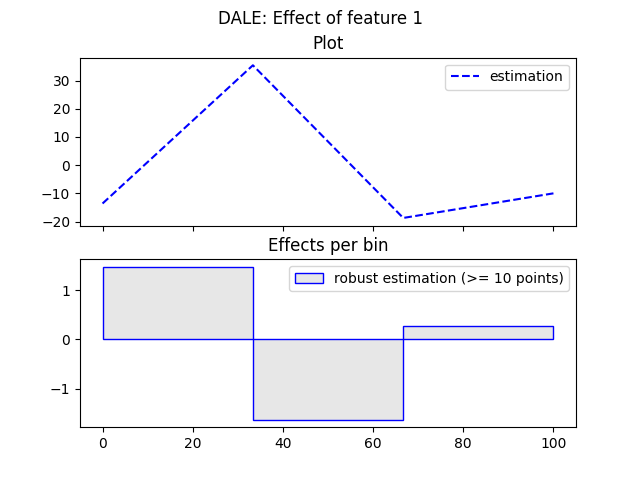
\includegraphics[width=.49\linewidth]{bullet_1/im_1.png}
  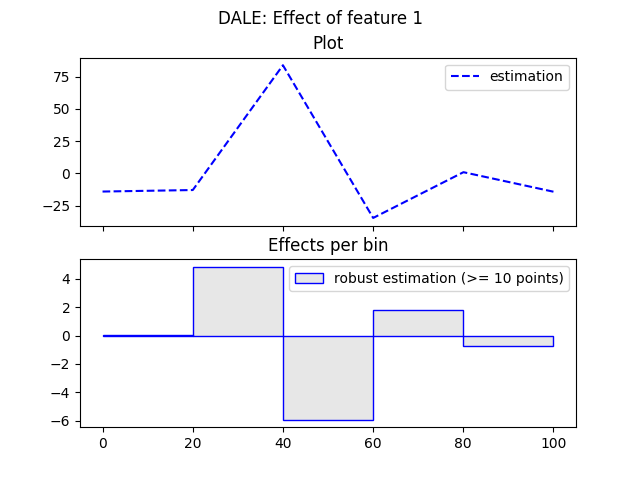
\includegraphics[width=.49\linewidth]{bullet_1/im_2.png}\\
  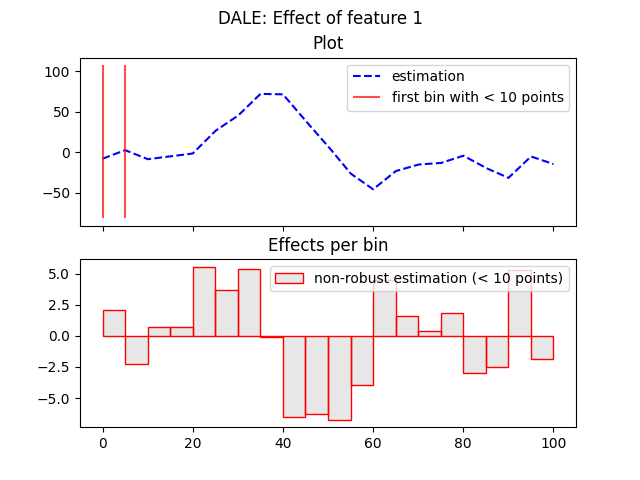
\includegraphics[width=.49\linewidth]{bullet_1/im_3.png}
  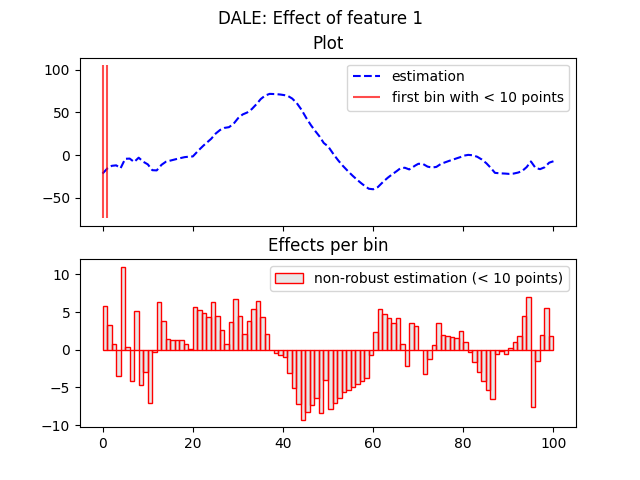
\includegraphics[width=.49\linewidth]{bullet_1/im_4.png}
  \caption{DALE effect for (a) \(K = 3\), (b) \(K = 5\), (c)
    \(K = 20\), (d) \(K = 100\)}
  \label{fig:bullet-1-im-1}
\end{figure}

\subsubsection*{Proposal}

We propose standard error as a metric for informing \textbf{to what extend
we should trust the feature effect plot}. \textbf{Standard error
  shows the expected error in the computation of the feature effect
  plot.} However, there are some constraints we must notice:

\begin{enumerate}
\item Our computations are based on the hypothesis that inside all
  bins \textbf{the gradient wrt. to the feature of interest doesn't
    depend on the value feature of interest}. In our example, in the
  interval \([0,20)\) the gradient is \(x_2 + 0.3\) (independent of
  \(x_2\)). But in the interval \([0,40)\) the gradient is 0.3 if
  \(x_1 < 20\) and 7 otherwise (not independent of
  \(x_2\)). Unfortunately, we cannot when this is the case. We just
  know that as the bins grow larger, it is more possible to violated
  this hypothesis, as in Figure~\ref{fig:bullet-1-im-2}(a). In this
  case both the ALE effect and the standard error are wrong.
\item The standard error should be trusted when it is estimated by a
  large of data points. For example, in plots (c) and (d), there are
  bins with less than 10 points. Therefore, in these cases, we cannot
  trust the plot or the standard error.
\item For being confident about the feature effect plot, we should
  check the region covered by 2 or 3 times the standard error. For
  example in~\ref{fig:bullet-1-im-2}, we observe that in plots (a) and
  (b), the green region showing the standard error is very big (covers
  the region from almost -100 to 100). Therefore, the effect cannot be
  trusted.
\end{enumerate}

\begin{figure}[!h]
  \centering
  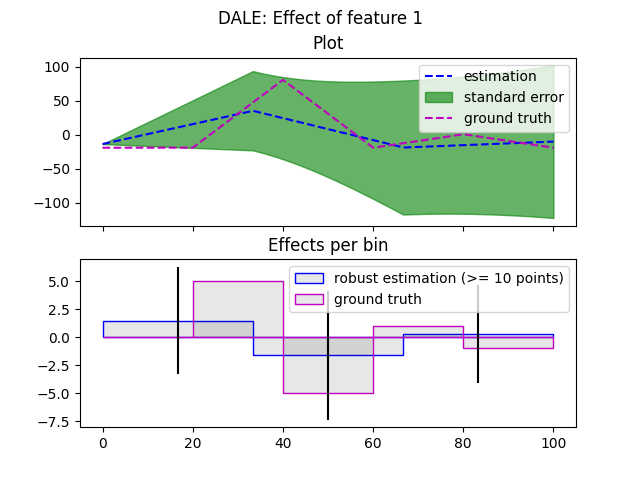
\includegraphics[width=.49\linewidth]{bullet_1/im_5.png}
  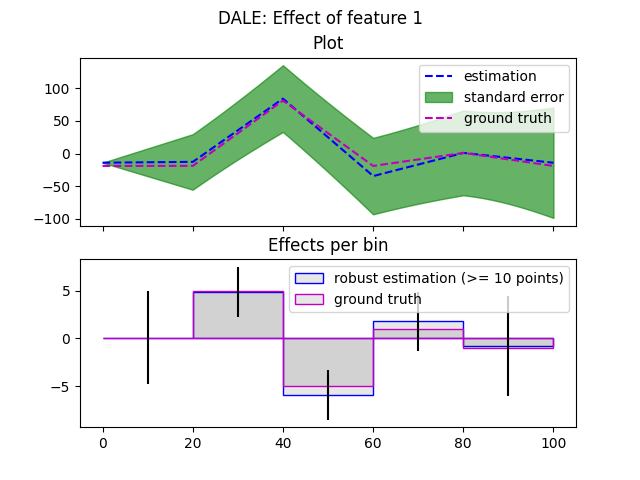
\includegraphics[width=.49\linewidth]{bullet_1/im_6.png}\\
  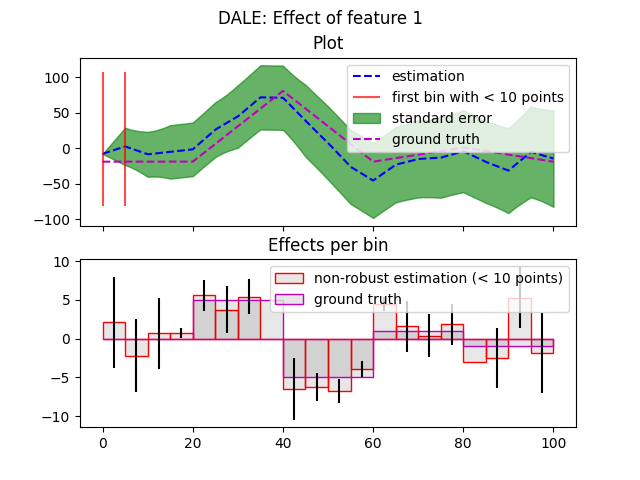
\includegraphics[width=.49\linewidth]{bullet_1/im_7.png}
  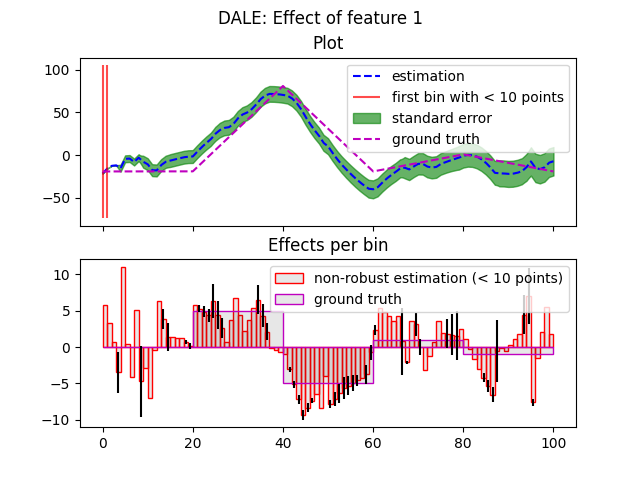
\includegraphics[width=.49\linewidth]{bullet_1/im_8.png}
  \caption{DALE effect with standard error for (a) \(K = 3\), (b)
    \(K = 5\), (c) \(K = 20\), (d) \(K = 100\)}
  \label{fig:bullet-1-im-2}
\end{figure}

If the above criteria are met, the standard error is a useful
metric. For example, if we repeat the experiment with a bigger dataset
\( (N = 10000) \) points, we get the results of figure
\ref{fig:bullet-1-im-3}. We observe that standard error gives accurate
trustability regions, in all plots, i.e. (b), (c), (d), apart from
(a). In (a), (b) and (c), it correctly us to trust the feature effect
plots. Misleadingly, it also informs to trust plot (a), which is
wrong. This because in this case, the first constraint has been
violated.


\begin{figure}[!h]
  \centering
  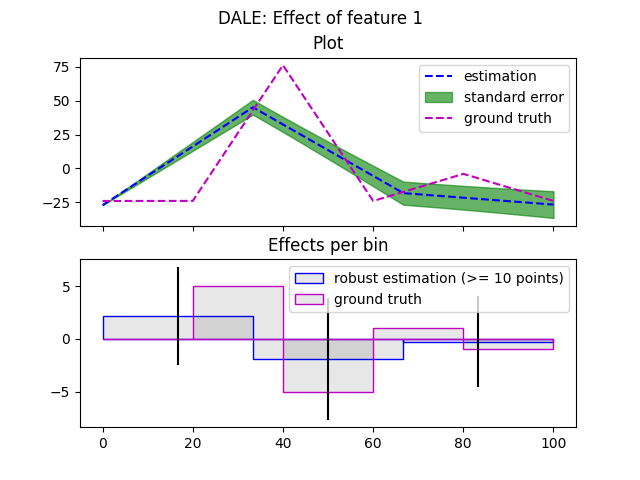
\includegraphics[width=.49\linewidth]{bullet_1/im_9.png}
  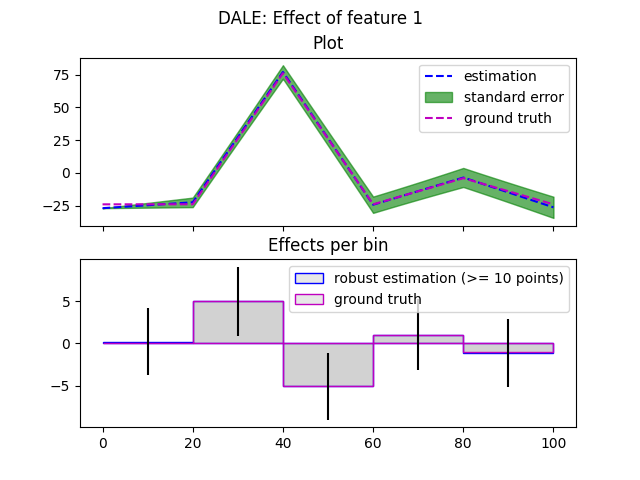
\includegraphics[width=.49\linewidth]{bullet_1/im_10.png}\\
  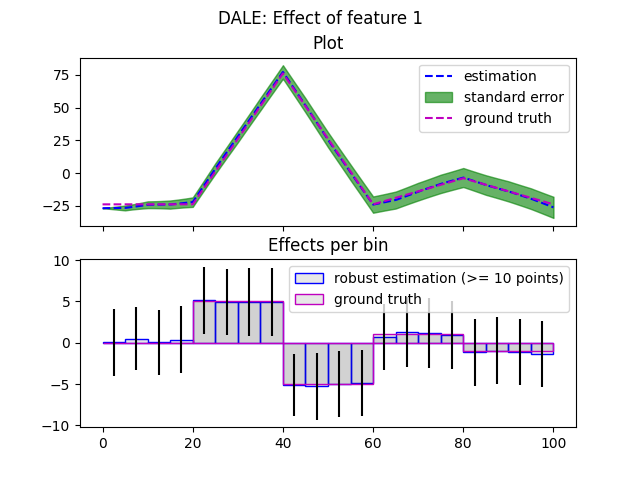
\includegraphics[width=.49\linewidth]{bullet_1/im_11.png}
  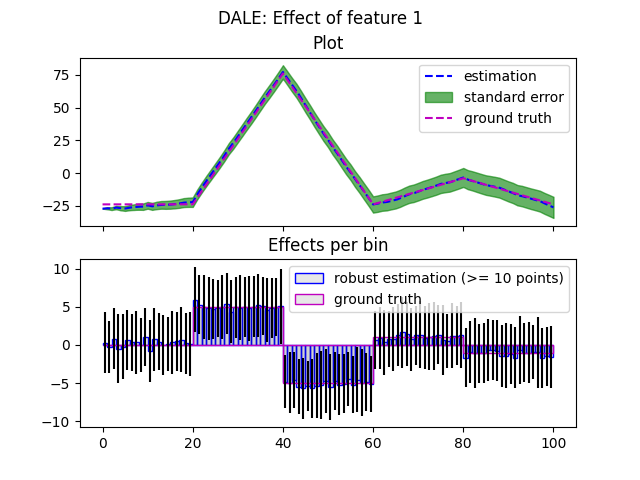
\includegraphics[width=.49\linewidth]{bullet_1/im_12.png}
  \caption{DALE effect with standard error for (a) \(K = 3\), (b)
    \(K = 5\), (c) \(K = 20\), (d) \(K = 100\)}
  \label{fig:bullet-1-im-3}
\end{figure}

\subsubsection*{Conclusion}

If the user can create small bins, i.e. (\(dx\) small enough
\(\rightarrow K \) big enough, to respect constraint 1 and has enough
points inside each bin (constraint 2), then the standard error reveals
to what extend we can trust the feature effect plot.

\section{Choose the more accurate feature effect plot to trust}

\subsubsection*{Statement}

Apart from having a metric of uncertainty about the feature effect
plot (standard error), we must also have a metric to choose the most
accurate feature effect plot.

\subsubsection*{Proposal}

We propose the minimization of the accumulated standard deviation (or
accumulated variance). For ALE with K bins, let's notate as:

\begin{itemize}
\item \(dx^K\) the length of each bin
\item \(p_i^K \) the number of the training points inside the \(i-th\) bin
\item \(\sigma_i^K \) the std of the local effects of the training points inside the \(i-th\) bin
\end{itemize}
%
We will minimize:

\begin{align} \label{eq:min-criterion}
  K_{min} &= \text{argmin}_{K} \quad  [dx^K  \sum_i^K \sigma_i^K * (1 - d_i^K)]\\
  & \text{s.t. } p_i^K \geq \texttt{min\_points\_per\_bin } \forall i
\end{align}
%
where \(d_i^K = 0.2 * \frac{p_i^K}{N} \in [0,0.1] \) works as a `discount', favoring the
creation of bigger bins in cases of similar standard deviation.

\subsubsection*{Example}

Let's see how the proposed metric works in the example of Chapter
2. We set \texttt{min\_points\_per\_bin = 10}. We repeat the procedure
for different number of points \(N=50, 100, 1000, 10000\). The results
are shown in \ref{fig:bullet-2-im-1}. For \(N=50\) we can evaluate the
loss only up to 4 bins (3 is the best) and for \(N=100\) up to 7 (5 is
the best). In all other cases 5 bins is the best solution (sensible),
with all multiples of 5 are also good options. All results make sense.


\begin{figure}[!h]
  \centering
  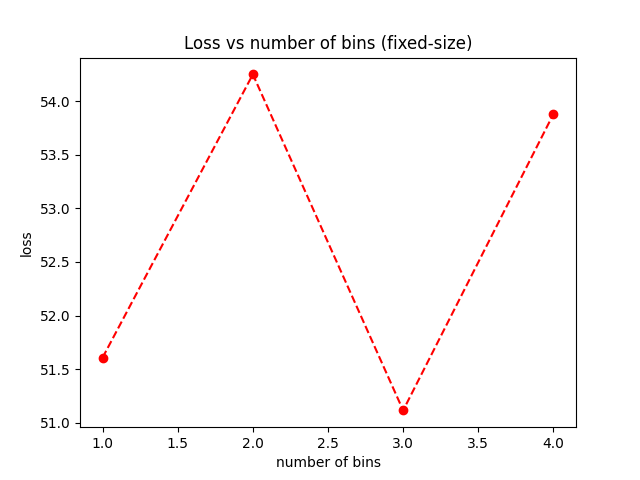
\includegraphics[width=.49\linewidth]{bullet_2/im_1.png}
  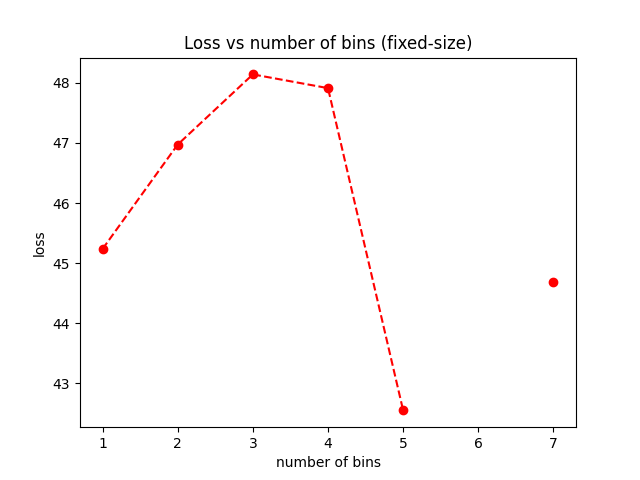
\includegraphics[width=.49\linewidth]{bullet_2/im_2.png}\\
  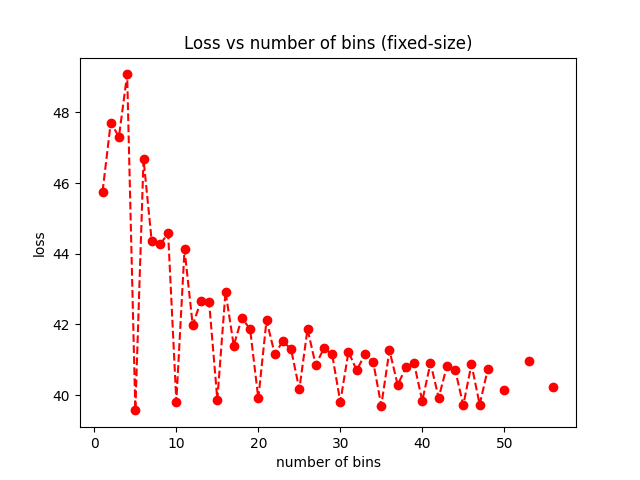
\includegraphics[width=.49\linewidth]{bullet_2/im_3.png}
  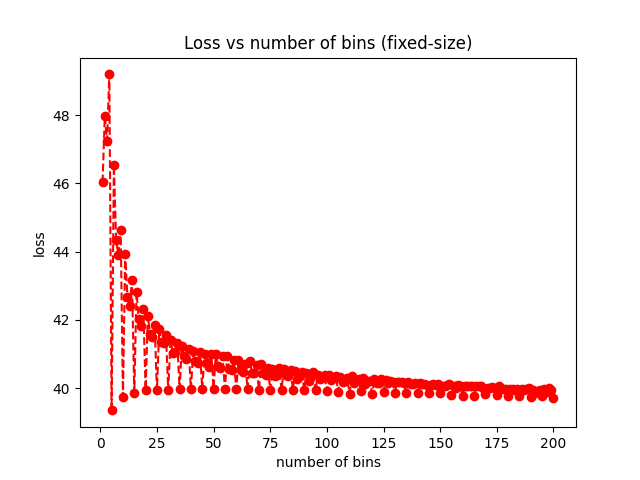
\includegraphics[width=.49\linewidth]{bullet_2/im_4.png}
  \caption{Loss (=accumulated standard error) for datasets of size (a)
    \(N = 50\), (b) \(N = 100\), (c) \(N = 1000\), (d) \(N = 10000\)}
  \label{fig:bullet-2-im-1}
\end{figure}


\subsubsection*{Conclusion}

Minimizing the accumulated standard deviation is a good indicator for
choosing the most accurate feature effect plot.

\section{Variable-size bins are important in many cases}

\subsubsection*{Statement}

Spliting the space in equally sized-bins is not always a good option.

\subsubsection*{Example}

Let's see the example of Figure \ref{fig:bullet-3-im-1}, where the
ground truth effect is a piecewise linear function with 3 parts. There
are two problems with applying equally-sized bins:

\begin{itemize}
\item The first two parts have length 20, whereas the third part has
  length 60. For capturing the first two effects we need
  \(dx \leq 20\), but this resolution adds noise to the third bin that
  could be bigger.
\item the data points are not uniformly split along the axis. From
  x=40 until x=100, they are sparse. This makes it difficult to split
  the space, with many bins since we won't have enough points per bin.
\end{itemize}

Therefore as we can see in figure \ref{fig:bullet-3-im-2}, with a
threshold of \(min\_points\_per\_bin = 10\), we can evaluate until
\(K=4\), which has the best loss. As we see, \(K=4\) has lower
resolution than needed, badly estimating feature effect (Figure
\ref{fig:bullet-3-im-2}(b)).

\begin{figure}[!h]
  \centering
  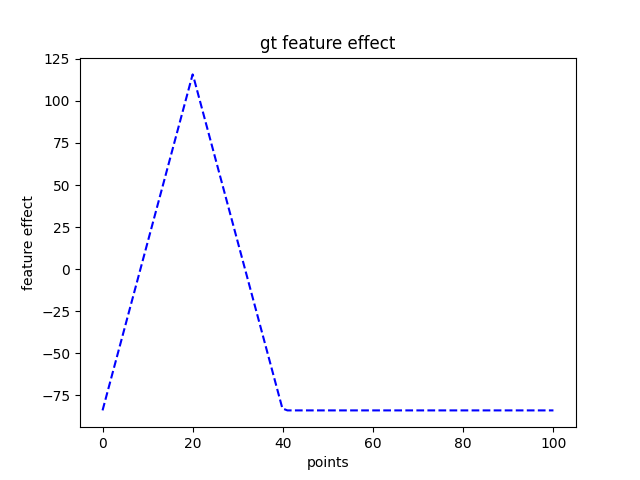
\includegraphics[width=.49\linewidth]{bullet_3/im_1.png}
  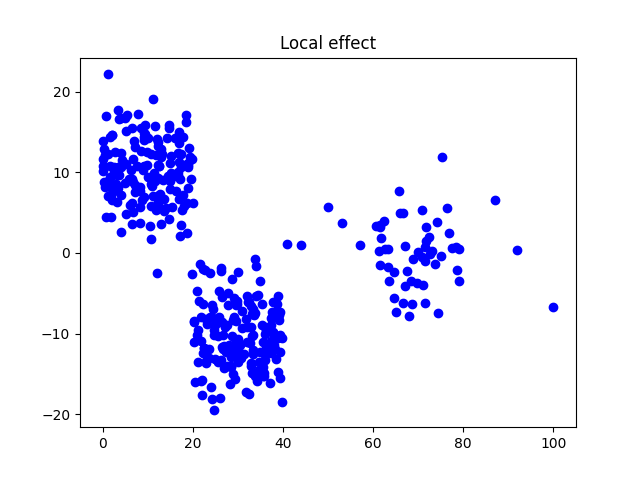
\includegraphics[width=.49\linewidth]{bullet_3/im_2.png}\\
  \caption{Left: Ground truth feature effect plot, Right: local effect
    for each point}
  \label{fig:bullet-3-im-1}
\end{figure}

\begin{figure}[!h]
  \centering
  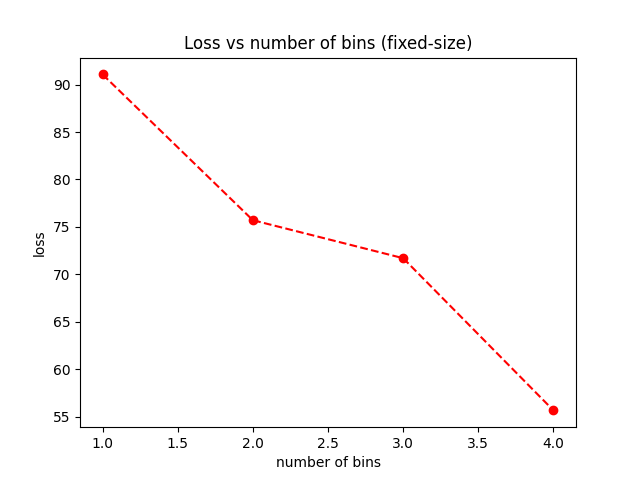
\includegraphics[width=.49\linewidth]{bullet_3/im_3.png}
  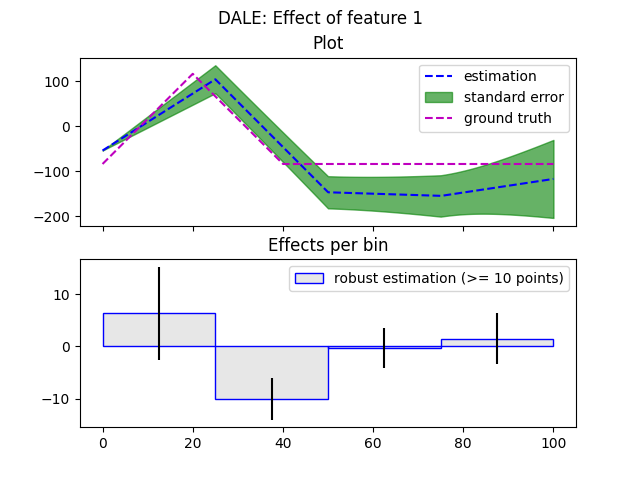
\includegraphics[width=.49\linewidth]{bullet_3/im_4.png}\\
  \caption{Left: Ground truth feature effect plot, Right: local effect for each point}
  \label{fig:bullet-3-im-2}
\end{figure}

\subsubsection*{Proposal}

We propose the creation of variable-size bins. The objective is the
minimisation of the loss as described in Section 3. In our example,
the algorithm created 5 bins (figure \ref{fig:bullet-3-im-3} (a)) that
lead to the feature effect of (figure \ref{fig:bullet-3-im-3} (b)),
which is almost perfect.

\begin{figure}[!h]
  \centering
  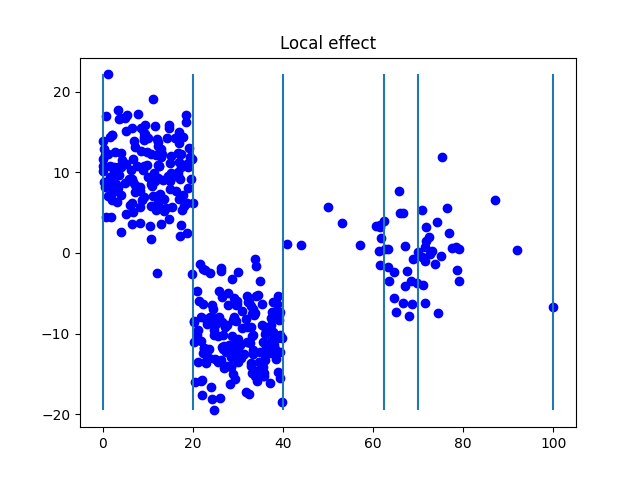
\includegraphics[width=.49\linewidth]{bullet_3/im_5.png}
  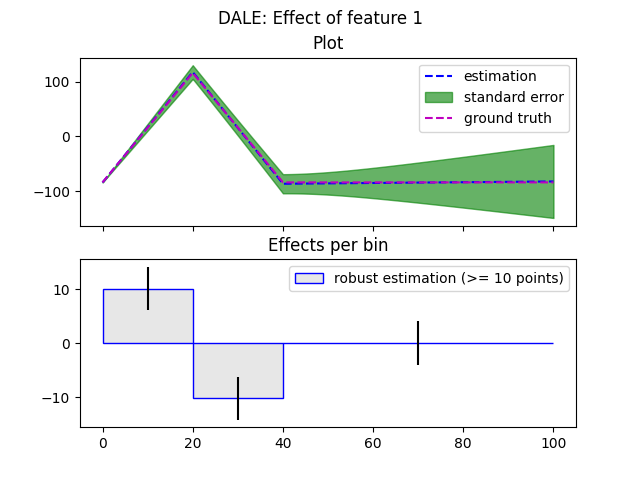
\includegraphics[width=.49\linewidth]{bullet_3/im_7.png}\\
  \caption{Left: Ground truth feature effect plot, Right: local effect for each point}
  \label{fig:bullet-3-im-3}
\end{figure}

\subsubsection*{Conclusion}

\section{Variable-size bins in case of non-linear feautre effects}

\subsubsection*{Statement}

The combination of non-linear and linear parts makes variable-size
feature effect even more important.

\begin{itemize}
\item If we have enough samples, we need small bins to approach
  accurately the non-linear parts.
\item We need wider bins for robust estimation of the linear parts
\end{itemize}

\subsubsection*{Example}

We define the following model:

\begin{equation} \label{eq:bullet-4-model}
  f(x_1, x_2) = 10x_1x_2 +
  \begin{cases}
    sinc(\pi x_1^2)  &,  0  \leq x_1 < \tau \\
    sinc(\pi \tau^2) &, \tau \leq x_1 \leq 5
  \end{cases}
\end{equation}
%
where \(x_1 \perp x_2 \Rightarrow p(x_1, x_2) = p(x_1)p(x_2)\) and \(\tau = 2.65\). The data generation distribution for \(x_1\) is:

\begin{equation} \label{eq:bullet-4-generative-x-1}
  p(x_1) =
  \begin{cases}
    \mathcal{U}(x_1; 0 , \tau)/2  &,  0  \leq x_1 < \tau \\
    \mathcal{N}(x_1; \mu = (5 + \tau)/2 , \sigma=0.3)/2 &, \tau \leq x_1 \leq 5
  \end{cases}
\end{equation}

and for \(x_2\):

\begin{equation} \label{eq:bullet-4-generative-x-2}
  p(x_2) = \mathcal{N}(x_2; \mu = 0 , \sigma=0.1)
\end{equation}

Therefore, the gradients wrt. \(x_1\) are:

\begin{equation} \label{eq:bullet-4-data-effect}
  \frac{\partial f}{ \partial x_1} (x_1) = 10x_2 +
  \begin{cases}
    2 \frac{\cos(\pi x_1^2)}{x_1} - 2 \frac{\sin(\pi x_1^2)}{\pi x_1^3}  &,  0  \leq x_1 < \tau \\
    0   &, \tau \leq x_1 \leq 5
  \end{cases}
\end{equation}
%
where \(x_2 \sim \mathcal{N}(\mu=0, \sigma=4)\). The ground truth ALE is:

\begin{equation} \label{eq:bullet-4-gt-ale}
  f_{\mathtt{ALE}}(x_s) = c +
  \begin{cases}
    sinc(\pi x_1^2)  &,  0  \leq x_1 < \tau \\
    sinc(\pi \tau^2)  &,  0  \leq x_1 < \tau \\
  \end{cases}
\end{equation}
%
where \(c\) is a normalizing constant. We generate N = 1000 data
points. In figure~\ref{fig:bullet-4-im-1}, we see the data points with
their respective gradients. In figure~\ref{fig:bullet-4-im-2}, we see
the fixed-size ALE plots; if we set \(K=50\), we capture the
non-linear parts in the first half, but we fail in linear second
part. Furthermore, we have empty bins, so we cannot trust the plot and
the standard error on the second half. The largest number of bins with
more than ten points in each bin, is \(K=5\) which fails to capture
the high-resolution effects. Variable size bins solves both problems
and provides the correct feature-effect.

\begin{figure}[!h]
  \centering
  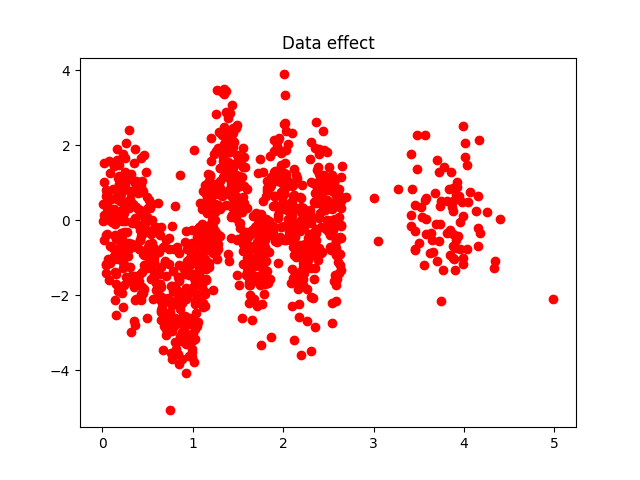
\includegraphics[width=.49\linewidth]{bullet_4/im_1.png}
  \caption{Data points with their gradients}
  \label{fig:bullet-4-im-1}
\end{figure}

\begin{figure}[!h]
  \centering
  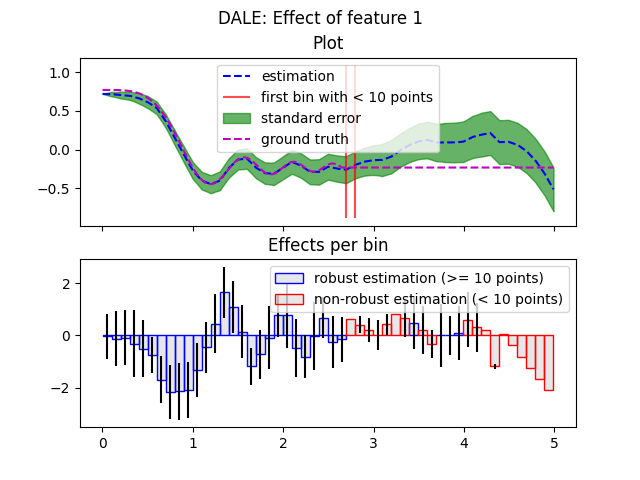
\includegraphics[width=.48\linewidth]{bullet_4/im_2.png}
  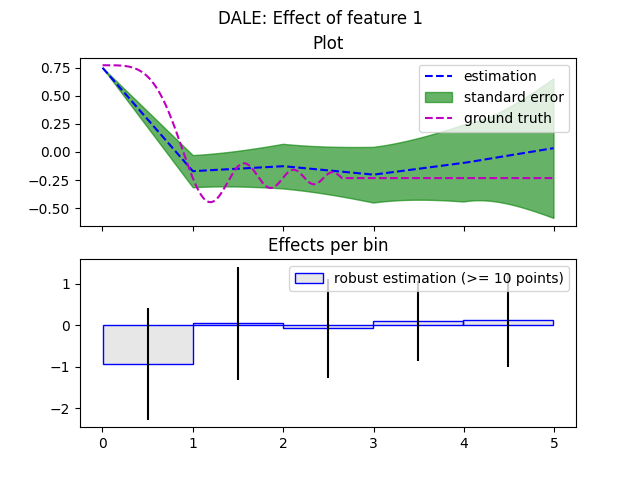
\includegraphics[width=.48\linewidth]{bullet_4/im_3.png}
  \caption{Fixed-size bins feature effect. Left: with K=50 and Right: with K=5.}
  \label{fig:bullet-4-im-2}
\end{figure}

\begin{figure}[!h]
  \centering
  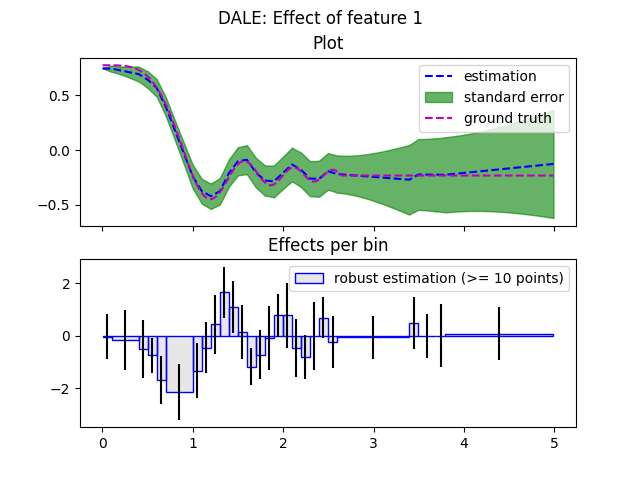
\includegraphics[width=.75\linewidth]{bullet_4/im_4.png}
  \caption{Variable-size bins.}
  \label{fig:bullet-4-im-3}
\end{figure}


\subsubsection*{Proposal}




\subsubsection*{Conclusion}

\end{document}
